\documentclass[aspectratio=169]{beamer}

\usefonttheme[onlymath]{serif}

\usepackage{physics}
\usepackage[export]{adjustbox}
\usepackage[absolute,overlay]{textpos}
\usepackage{graphicx}

\usepackage{derivative}
% I should not have to do this
\DeclareOdvVariant{\odv}{d}[style-inf=\mathrm] 



\begin{document}
    \begin{frame}
        \frametitle{Question}
        \begin{textblock}{6}(8.5, 4)
            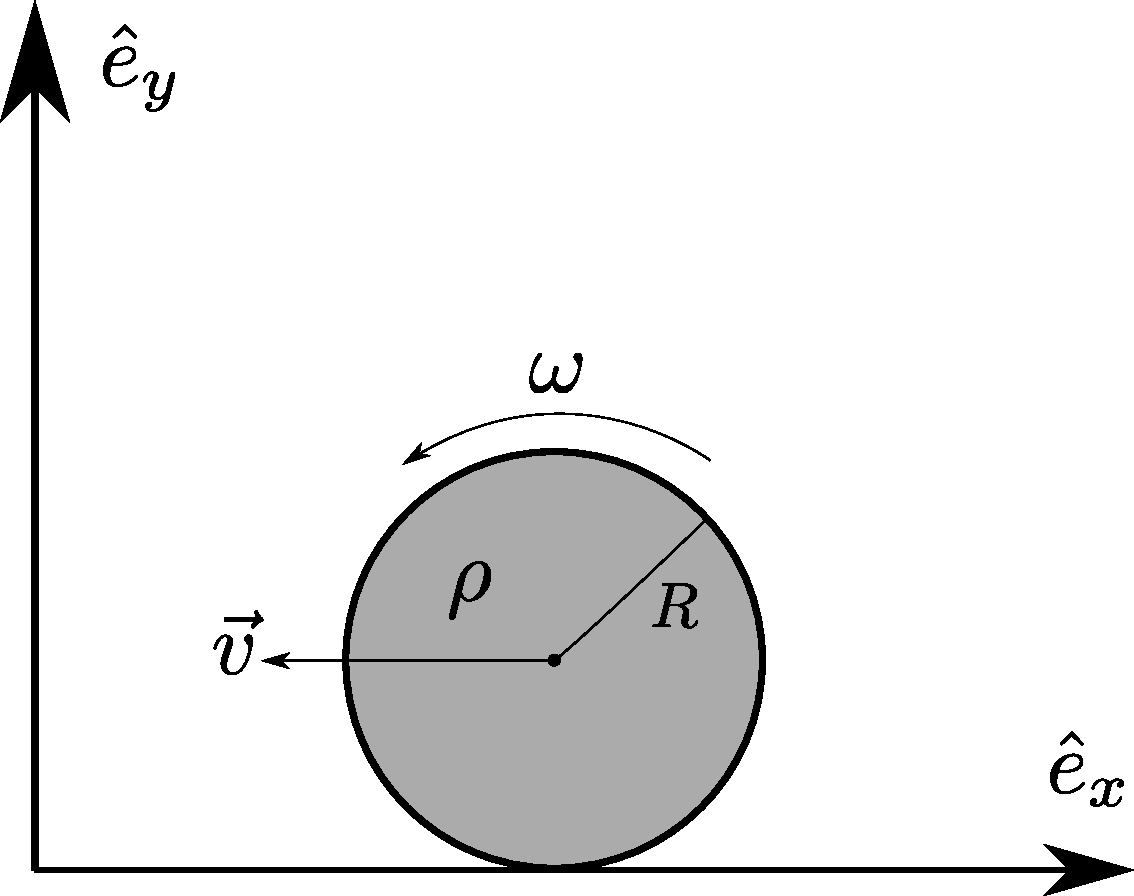
\includegraphics[width=\textwidth]{ball_setup.pdf}
        \end{textblock}
        \begin{itemize}
            \item Sphere of density $\rho$, radius $R$ with \\velocity $\vec v = - v_0 \hat e_x$.
            \item Hit wall, bounces elastically and without\\ slipping
            \item What is velocity $\vec v'$ after collision, and\\ how does it depend on $v_0$, $\rho$ and $R$?\\ What happens for small $R$?
            \item What if sphere is hollow?
        \end{itemize}
    \end{frame}

    \begin{frame}
        \frametitle{Quantities}
        \begin{textblock}{6}(8.5, 4)
            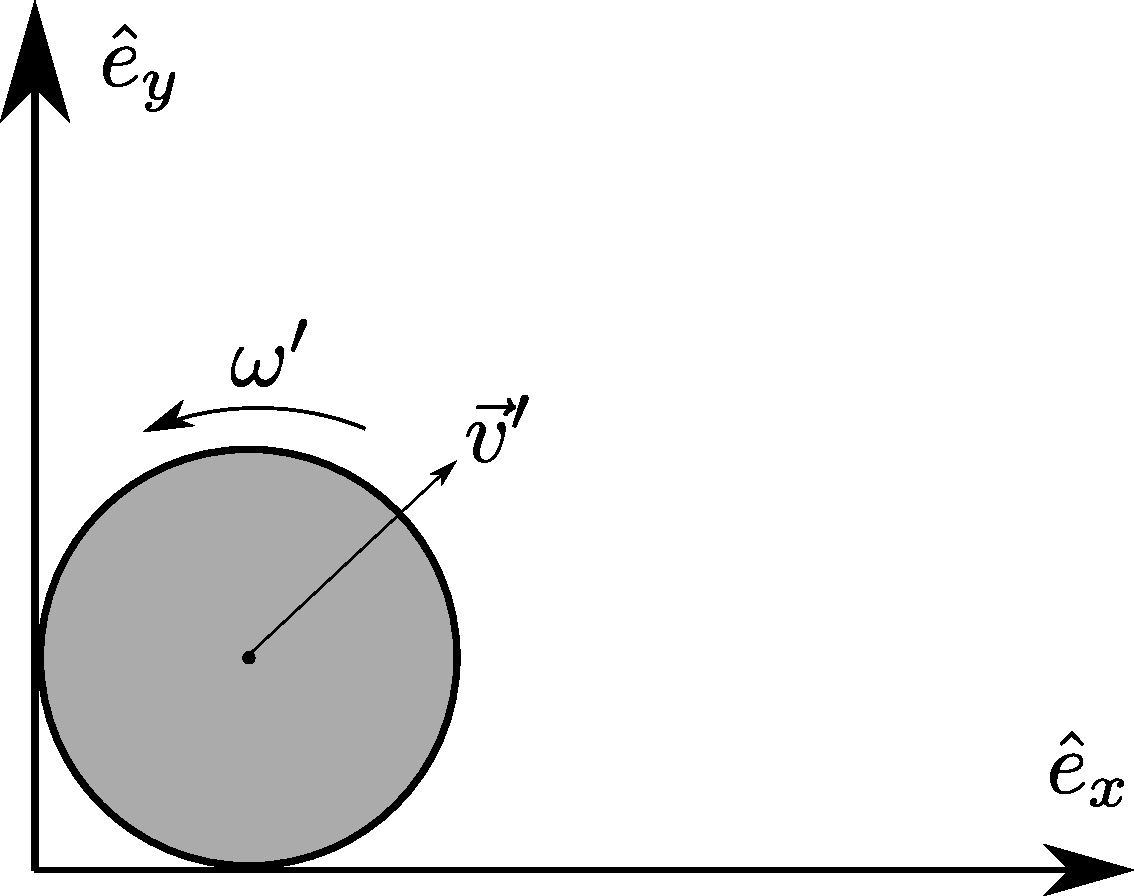
\includegraphics[width=\textwidth]{ball_collision.pdf}
        \end{textblock}
        \begin{itemize}
            \item Angular velocity: $\omega$
            \item Mass: $m = \frac{4 \pi}{3} \rho R^3$.
            \item Moment of inertia: $I = \frac{2}{5} m R^2$.
            \item After: $\omega'$, $\vec v' = v_x \hat e_x + v_y \hat e_y$.
        \end{itemize}
    \end{frame}


    \begin{frame}
        \frametitle{Conditions}
        \begin{itemize}
            \item No slip at ground: $\omega = \frac{v_0}{R}$.
            \item No slip at collision: $\omega' = \frac{v_y}{R}$.
            \item Energy:
            $$
            E = \frac{1}{2} m |\vec v|^2 + \frac{1}{2} I \omega^2
            = \frac{1}{2} \frac{7}{5} m v_0^2,
            $$
            $$
            E' = \frac{1}{2} m |\vec v'|^2 + \frac{1}{2} \frac{I}{R^2} \omega'^2
            = \frac{1}{2}m \left( v_x^2 + \frac{7}{5} v_y^2 \right) 
            $$
            \item Elasticity: 
            $$
                E = E' \implies
                v_0^2 = \frac{5}{7}v_x^2 + v_y^2
            $$
        \end{itemize}
    \end{frame}

    \begin{frame}
        \frametitle{Conservation of angular momentum}
        \begin{itemize}
            \item Angular momentum around point of collision: No arm, no torque, conservation of angular momentum.
            \item Before collision: No angular momentum from center-of-mass motion, only spin angular momentum:
            $|\vec L| = I \omega = \frac{2}{5} m v_0 R $.
            \item After, additional term from $y$ component of velocity: 
            $|\vec  L'| = I \omega' + mv_y R = \frac{7}{5} m v_y R$.
            \item Conservation of angular momentum, $\vec L = \vec L'$,
            $
                \implies v_y = \frac{2}{7} v_0.
            $
        \end{itemize}
    \end{frame}

    \begin{frame}
        \frametitle{Solution}
        
        \begin{itemize}
            \item Combining gives
            $$
                v_0^2 = \frac{5}{7} v_x^2 + \left(\frac{2}{7}\right)^2 v_0^2
                \implies v_x^2 = \frac{9}{7} v_0^2
            $$
            \item Finally 
            $$
                \vec v' = v_0 \left( \frac{3}{\sqrt 7}\hat e_x + \frac{2}{7} \hat e_y\right)
                \approx v_0(1.13 \hat e_x + 0.29 \hat e_y)
            $$
            \item Independent of $\rho, R$ --- no other constants of same dimension, scale free.
        \end{itemize}
    \end{frame}

    \begin{frame}
        \frametitle{Hollow sphere}
        
        \begin{itemize}
            \item Only difference: new moment of inertia $I = \frac{2}{3} m r^2$
            \item $v_0^2 = \frac{3}{5}v_x^2 + v_y^2$, $v_y = \frac{2}{5}v_0$, \\
            $$
                \implies \vec v' = v_0 \left(  \sqrt{\frac{7}{5}} \hat e_x + \frac{2}{5} \hat e_y\right)
                \approx v_0(1.18 \hat e_x + 0.4 \hat e_y)
            $$
        \end{itemize}
    \end{frame}

\end{document}